% Author: Izaak Neutelings (September 2020)
% Inspiration: https://tex.stackexchange.com/questions/25531/adding-underbrace-in-tikz
\documentclass[border=3pt,tikz]{standalone}
\usepackage{physics}
\usepackage{ifthen}
\usepackage{tikz}
\usetikzlibrary{patterns,snakes}
\tikzset{>=latex} % for LaTeX arrow head

\colorlet{myred}{red!65!black}
\colorlet{acol}{red!50!blue!80!black!80}
\tikzstyle{ground}=[preaction={fill,top color=black!10,bottom color=black!5,shading angle=20},
                    fill,pattern=north east lines,draw=none,minimum width=0.3,minimum height=0.6]
\tikzstyle{mass}=[line width=0.6,red!30!black,fill=red!40!black!10,rounded corners=1,
                  top color=red!40!black!20,bottom color=red!40!black!10,shading angle=20]
\tikzstyle{rope}=[brown!70!black,line width=1.2,line cap=round] %very thick

% FORCES SWITCH
\tikzstyle{force}=[->,myred,thick,line cap=round]
\newcommand{\vbF}{\vb{F}}
\newboolean{showforces}
\setboolean{showforces}{true}


\begin{document}


% HORIZONTAL ground
\begin{tikzpicture}
  \def\W{2.0} % ground width
  \def\D{0.2} % ground depth
  \def\h{0.6} % mass height
  \def\w{0.8} % mass width
  \draw[ground] (-\W/2,0) rectangle++ (\W,-\D);
  \draw (-\W/2,0) --++ (\W,0);
  \draw[mass] (-\w/2,0) rectangle++ (\w,\h) node[midway] {$m$};
  \ifthenelse{\boolean{showforces}}{
    \draw[->] (1.0*\w,0.5*\h) --++ (0,0.9*\h) node[below=4,right=0] {$y$};
    \draw[force] (-0.3*\w,0.0*\h) --++ (0, 1.4*\h) node[left] {$\vbF_\mathrm{N}$};
    \draw[force] ( 0.3*\w,0.5*\h) --++ (0,-1.4*\h) node[right=5,below=-3] {$\vbF_\mathrm{g} = -mg\vu{y}$};
    %\draw[force] (0,0.9*\h) --++ (0, 1.0*\h) node[left] {$\vbF_\mathrm{N}$};
    %\draw[force] (0,0.1*\h) --++ (0,-1.0*\h) node[right=5,below=-2] {$\vbF_\mathrm{g} = -mg\vu{y}$};
  }{}
\end{tikzpicture}


% HORIZONTAL ground - lift
\begin{tikzpicture}
  \def\W{2.1}  % ground width
  \def\D{0.2}  % ground depth
  \def\h{0.6}  % mass height
  \def\w{0.7}  % mass width
  \def\H{2.0}  % human height
  \def\mx{-0.12*\W} % mass x coordinate
  
  % SETUP
  \draw[ground] (-\W/2,0) rectangle++ (\W,-\D);
  \draw (-\W/2,0) --++ (\W,0);
  \draw[rope]  (\mx,\h) -- (\mx*0.98,0.6*\H) coordinate (RH);
  \draw[mass] (\mx-\w/2,0) rectangle++ (\w,\h) node[midway] {$m$};
  
  % FORCES
  \ifthenelse{\boolean{showforces}}{
    \draw[->] (0.42*\W,0.5*\h) --++ (0,0.9*\h) node[below=4,right=0] {$y$};
    \draw[force] (\mx-0.15*\w,0.9*\h) --++ (0, 1.0*\h) node[above left=-3] {$\vbF$};
    \draw[force] (\mx-0.35*\w,0.0*\h) --++ (0, 0.7*\h) node[left] {$\vbF_\mathrm{N}$};
    \draw[force] (\mx+0.30*\w,0.5*\h) --++ (0,-1.4*\h) node[right=5,below=-2] {$\vbF_\mathrm{g} = -mg\vu{y}$};
  }{}
  
  % PERSON
  \draw[thick] (0.17*\W,\H) circle (0.3) coordinate (H);
  \draw[thick] (H)++(-90:0.3) coordinate (N) to[out=-85,in=85]++ (0,-0.40*\H) coordinate (P);
  \draw[thick,line cap=round] (N)++(-85:0.03) to[out=-115,in=3] (RH);
  \draw[thick,line cap=round] (N)++(-85:0.03) to[out=-60,in=90]++ ( 0.08*\W,-0.4*\H);
  \draw[thick] (P) to[out=-110,in=85] (0.09*\W,0);
  \draw[thick] (P) to[out=-80,in=108] (0.23*\W,0);
  
\end{tikzpicture}


% FRICTION static/dynamical
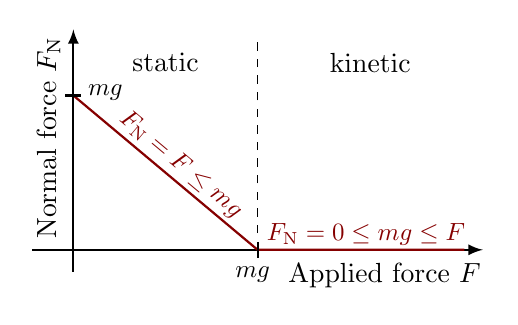
\begin{tikzpicture}
  \def\xmax{5.2}
  \def\ymax{2.8}
  \def\xc{0.45*\xmax}
  \def\yc{0.7*\ymax}
  \draw[->,thick] (-0.1*\xmax,0) -- (\xmax,0) node[right=4,below left=1] {Applied force $F$};
  \draw[->,thick] (0,-0.1*\ymax) -- (0,\ymax) node[above left=1,rotate=90] {Normal force $F_\mathrm{N}$};
  \draw[dashed] (\xc,0) --++ (0,0.97*\ymax); % coordinate (C);
  \draw[myred!80!black,thick]
    (0,\yc) -- (\xc,0)
    node[scale=0.9,midway,right=1,above=-3,rotate={-atan2(\yc,\xc)}] {$F_\mathrm{N} = F \leq mg$}
    --++ (\xmax-1.1*\xc,0)
    node[scale=0.9,midway,right=2,above=-2] {$F_\mathrm{N} = 0 \leq mg \leq F$};
  \draw[thick] (\xc,0.1) --++ (0,-0.2) node[scale=0.9,left=2,below] {$mg$};
  \draw[thick] (-0.1,\yc) --++ (0.2,0) node[scale=0.9,above=1,right=-1] {$mg$};
  \node[] at (\xc/2,0.85*\ymax) {static};
  \node[] at ({(\xmax+\xc)/2},0.85*\ymax) {kinetic};
  
\end{tikzpicture}


% NORMAL FORCE - balance
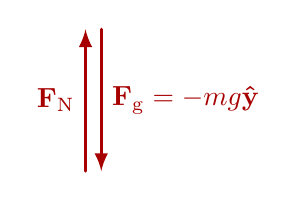
\begin{tikzpicture}
  \def\F{1.8}
  \draw[force,very thick] (0,0) -- (0,\F) node[midway,left=0] {$\vbF_\mathrm{N}$};
  \draw[force,very thick] (0.2,\F) --++ (0,-\F) node[midway,right=0] {$\vbF_\mathrm{g}=-mg\vu{y}$};
\end{tikzpicture}


% NORMAL FORCE lift - balance
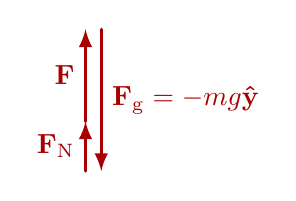
\begin{tikzpicture}
  \def\F{1.8}
  \draw[force,very thick] (0,0) -- (0,0.35*\F) node[midway,left=0] {$\vbF_\mathrm{N}$};
  \draw[force,very thick] (0,0.35*\F) -- (0,\F) node[midway,left=0] {$\vbF$};
  \draw[force,very thick] (0.2,\F) --++ (0,-\F) node[midway,right=0] {$\vbF_\mathrm{g}=-mg\vu{y}$};
\end{tikzpicture}


% NORMAL FORCE lift - acceleration
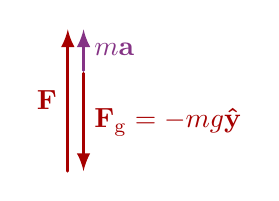
\begin{tikzpicture}
  \def\F{1.8}
  \draw[force,very thick] (0,0) -- (0,\F) node[midway,left=0] {$\vbF$};
  \draw[force,very thick] (0.2,0.689*\F) --++ (0.0,-0.689*\F) node[midway,right=0] {$\vbF_\mathrm{g}=-mg\vu{y}$};
  \draw[force,acol,very thick] (0.2,0.711*\F) --++ (0.0,0.289*\F) node[midway,right=0] {$m\vb{a}$};
\end{tikzpicture}


\end{document}